\epigraph{\emph{Je me détourne avec effroi et horreur de cette plaie lamentable des fonctions continues qui n'ont point de dérivées.}}{--- Charles \textsc{Hermite} (1893)}
    
\epigraph{\emph{C’est un cas où il est vraiment naturel de penser à ces fonctions continues sans dérivées que les mathématiciens ont imaginées, et que l’on regardait à tort comme de simples curiosités mathématiques, puisque l’expérience peut les suggérer.}}{--- Jean \textsc{Perrin} \footnote{Physicien, chimiste et homme politique français (1870 - 1942), prix Nobel de physique 1926.}, au sujet du mouvement brownien}
    
- thème Ch. 8 \\
- DS MPSI 2015 \\
- \url{https://share.miple.co/content/XEZ7y9BayeSN1} \\
- \url{http://christophebertault.fr/documents/articles/Article - Une famille nombreuse de fonctions continues partout derivables nulle part.pdf}

\begin{itemize}
    \item Intégrale à paramètre vs. série de fonctions
    \item Développements asymptotiques de sommes de séries de fonctions
\end{itemize}

\begin{marginfigure}[-5cm]
	% This file was created with tikzplotlib v0.10.1.
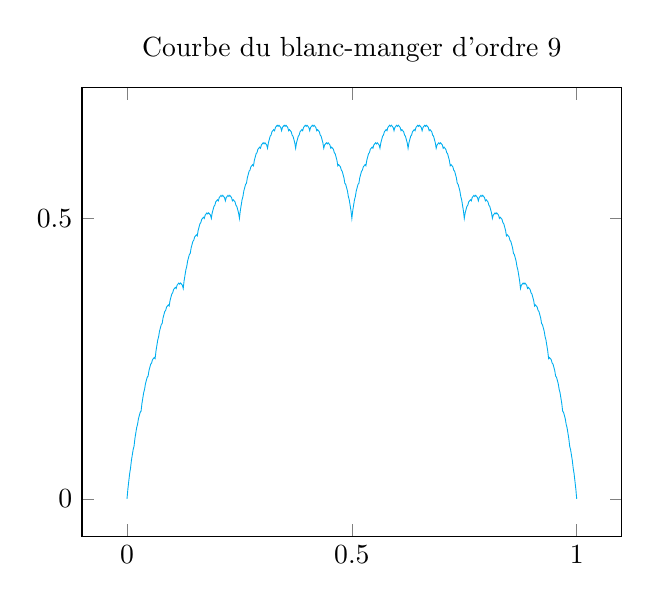
\begin{tikzpicture}

\begin{axis}[
title={Courbe du blanc-manger d'ordre 9},
xtick={0, 1/2, 1}, 
ytick={0, 1/2, 1}
]
\addplot [line width=0.32pt, cyan]
table {%
0 0
0.001953125 0.017578125
0.00390625 0.03125
0.005859375 0.044921875
0.0078125 0.0546875
0.009765625 0.068359375
0.01171875 0.078125
0.013671875 0.087890625
0.015625 0.09375
0.017578125 0.107421875
0.01953125 0.1171875
0.021484375 0.126953125
0.0234375 0.1328125
0.025390625 0.142578125
0.02734375 0.1484375
0.029296875 0.154296875
0.03125 0.15625
0.033203125 0.169921875
0.03515625 0.1796875
0.037109375 0.189453125
0.0390625 0.1953125
0.041015625 0.205078125
0.04296875 0.2109375
0.044921875 0.216796875
0.046875 0.21875
0.048828125 0.228515625
0.05078125 0.234375
0.052734375 0.240234375
0.0546875 0.2421875
0.056640625 0.248046875
0.05859375 0.25
0.060546875 0.251953125
0.0625 0.25
0.064453125 0.263671875
0.06640625 0.2734375
0.068359375 0.283203125
0.0703125 0.2890625
0.072265625 0.298828125
0.07421875 0.3046875
0.076171875 0.310546875
0.078125 0.3125
0.080078125 0.322265625
0.08203125 0.328125
0.083984375 0.333984375
0.0859375 0.3359375
0.087890625 0.341796875
0.08984375 0.34375
0.091796875 0.345703125
0.09375 0.34375
0.095703125 0.353515625
0.09765625 0.359375
0.099609375 0.365234375
0.1015625 0.3671875
0.103515625 0.373046875
0.10546875 0.375
0.107421875 0.376953125
0.109375 0.375
0.111328125 0.380859375
0.11328125 0.3828125
0.115234375 0.384765625
0.1171875 0.3828125
0.119140625 0.384765625
0.12109375 0.3828125
0.123046875 0.380859375
0.125 0.375
0.126953125 0.388671875
0.12890625 0.3984375
0.130859375 0.408203125
0.1328125 0.4140625
0.134765625 0.423828125
0.13671875 0.4296875
0.138671875 0.435546875
0.140625 0.4375
0.142578125 0.447265625
0.14453125 0.453125
0.146484375 0.458984375
0.1484375 0.4609375
0.150390625 0.466796875
0.15234375 0.46875
0.154296875 0.470703125
0.15625 0.46875
0.158203125 0.478515625
0.16015625 0.484375
0.162109375 0.490234375
0.1640625 0.4921875
0.166015625 0.498046875
0.16796875 0.5
0.169921875 0.501953125
0.171875 0.5
0.173828125 0.505859375
0.17578125 0.5078125
0.177734375 0.509765625
0.1796875 0.5078125
0.181640625 0.509765625
0.18359375 0.5078125
0.185546875 0.505859375
0.1875 0.5
0.189453125 0.509765625
0.19140625 0.515625
0.193359375 0.521484375
0.1953125 0.5234375
0.197265625 0.529296875
0.19921875 0.53125
0.201171875 0.533203125
0.203125 0.53125
0.205078125 0.537109375
0.20703125 0.5390625
0.208984375 0.541015625
0.2109375 0.5390625
0.212890625 0.541015625
0.21484375 0.5390625
0.216796875 0.537109375
0.21875 0.53125
0.220703125 0.537109375
0.22265625 0.5390625
0.224609375 0.541015625
0.2265625 0.5390625
0.228515625 0.541015625
0.23046875 0.5390625
0.232421875 0.537109375
0.234375 0.53125
0.236328125 0.533203125
0.23828125 0.53125
0.240234375 0.529296875
0.2421875 0.5234375
0.244140625 0.521484375
0.24609375 0.515625
0.248046875 0.509765625
0.25 0.5
0.251953125 0.513671875
0.25390625 0.5234375
0.255859375 0.533203125
0.2578125 0.5390625
0.259765625 0.548828125
0.26171875 0.5546875
0.263671875 0.560546875
0.265625 0.5625
0.267578125 0.572265625
0.26953125 0.578125
0.271484375 0.583984375
0.2734375 0.5859375
0.275390625 0.591796875
0.27734375 0.59375
0.279296875 0.595703125
0.28125 0.59375
0.283203125 0.603515625
0.28515625 0.609375
0.287109375 0.615234375
0.2890625 0.6171875
0.291015625 0.623046875
0.29296875 0.625
0.294921875 0.626953125
0.296875 0.625
0.298828125 0.630859375
0.30078125 0.6328125
0.302734375 0.634765625
0.3046875 0.6328125
0.306640625 0.634765625
0.30859375 0.6328125
0.310546875 0.630859375
0.3125 0.625
0.314453125 0.634765625
0.31640625 0.640625
0.318359375 0.646484375
0.3203125 0.6484375
0.322265625 0.654296875
0.32421875 0.65625
0.326171875 0.658203125
0.328125 0.65625
0.330078125 0.662109375
0.33203125 0.6640625
0.333984375 0.666015625
0.3359375 0.6640625
0.337890625 0.666015625
0.33984375 0.6640625
0.341796875 0.662109375
0.34375 0.65625
0.345703125 0.662109375
0.34765625 0.6640625
0.349609375 0.666015625
0.3515625 0.6640625
0.353515625 0.666015625
0.35546875 0.6640625
0.357421875 0.662109375
0.359375 0.65625
0.361328125 0.658203125
0.36328125 0.65625
0.365234375 0.654296875
0.3671875 0.6484375
0.369140625 0.646484375
0.37109375 0.640625
0.373046875 0.634765625
0.375 0.625
0.376953125 0.634765625
0.37890625 0.640625
0.380859375 0.646484375
0.3828125 0.6484375
0.384765625 0.654296875
0.38671875 0.65625
0.388671875 0.658203125
0.390625 0.65625
0.392578125 0.662109375
0.39453125 0.6640625
0.396484375 0.666015625
0.3984375 0.6640625
0.400390625 0.666015625
0.40234375 0.6640625
0.404296875 0.662109375
0.40625 0.65625
0.408203125 0.662109375
0.41015625 0.6640625
0.412109375 0.666015625
0.4140625 0.6640625
0.416015625 0.666015625
0.41796875 0.6640625
0.419921875 0.662109375
0.421875 0.65625
0.423828125 0.658203125
0.42578125 0.65625
0.427734375 0.654296875
0.4296875 0.6484375
0.431640625 0.646484375
0.43359375 0.640625
0.435546875 0.634765625
0.4375 0.625
0.439453125 0.630859375
0.44140625 0.6328125
0.443359375 0.634765625
0.4453125 0.6328125
0.447265625 0.634765625
0.44921875 0.6328125
0.451171875 0.630859375
0.453125 0.625
0.455078125 0.626953125
0.45703125 0.625
0.458984375 0.623046875
0.4609375 0.6171875
0.462890625 0.615234375
0.46484375 0.609375
0.466796875 0.603515625
0.46875 0.59375
0.470703125 0.595703125
0.47265625 0.59375
0.474609375 0.591796875
0.4765625 0.5859375
0.478515625 0.583984375
0.48046875 0.578125
0.482421875 0.572265625
0.484375 0.5625
0.486328125 0.560546875
0.48828125 0.5546875
0.490234375 0.548828125
0.4921875 0.5390625
0.494140625 0.533203125
0.49609375 0.5234375
0.498046875 0.513671875
0.5 0.5
0.501953125 0.513671875
0.50390625 0.5234375
0.505859375 0.533203125
0.5078125 0.5390625
0.509765625 0.548828125
0.51171875 0.5546875
0.513671875 0.560546875
0.515625 0.5625
0.517578125 0.572265625
0.51953125 0.578125
0.521484375 0.583984375
0.5234375 0.5859375
0.525390625 0.591796875
0.52734375 0.59375
0.529296875 0.595703125
0.53125 0.59375
0.533203125 0.603515625
0.53515625 0.609375
0.537109375 0.615234375
0.5390625 0.6171875
0.541015625 0.623046875
0.54296875 0.625
0.544921875 0.626953125
0.546875 0.625
0.548828125 0.630859375
0.55078125 0.6328125
0.552734375 0.634765625
0.5546875 0.6328125
0.556640625 0.634765625
0.55859375 0.6328125
0.560546875 0.630859375
0.5625 0.625
0.564453125 0.634765625
0.56640625 0.640625
0.568359375 0.646484375
0.5703125 0.6484375
0.572265625 0.654296875
0.57421875 0.65625
0.576171875 0.658203125
0.578125 0.65625
0.580078125 0.662109375
0.58203125 0.6640625
0.583984375 0.666015625
0.5859375 0.6640625
0.587890625 0.666015625
0.58984375 0.6640625
0.591796875 0.662109375
0.59375 0.65625
0.595703125 0.662109375
0.59765625 0.6640625
0.599609375 0.666015625
0.6015625 0.6640625
0.603515625 0.666015625
0.60546875 0.6640625
0.607421875 0.662109375
0.609375 0.65625
0.611328125 0.658203125
0.61328125 0.65625
0.615234375 0.654296875
0.6171875 0.6484375
0.619140625 0.646484375
0.62109375 0.640625
0.623046875 0.634765625
0.625 0.625
0.626953125 0.634765625
0.62890625 0.640625
0.630859375 0.646484375
0.6328125 0.6484375
0.634765625 0.654296875
0.63671875 0.65625
0.638671875 0.658203125
0.640625 0.65625
0.642578125 0.662109375
0.64453125 0.6640625
0.646484375 0.666015625
0.6484375 0.6640625
0.650390625 0.666015625
0.65234375 0.6640625
0.654296875 0.662109375
0.65625 0.65625
0.658203125 0.662109375
0.66015625 0.6640625
0.662109375 0.666015625
0.6640625 0.6640625
0.666015625 0.666015625
0.66796875 0.6640625
0.669921875 0.662109375
0.671875 0.65625
0.673828125 0.658203125
0.67578125 0.65625
0.677734375 0.654296875
0.6796875 0.6484375
0.681640625 0.646484375
0.68359375 0.640625
0.685546875 0.634765625
0.6875 0.625
0.689453125 0.630859375
0.69140625 0.6328125
0.693359375 0.634765625
0.6953125 0.6328125
0.697265625 0.634765625
0.69921875 0.6328125
0.701171875 0.630859375
0.703125 0.625
0.705078125 0.626953125
0.70703125 0.625
0.708984375 0.623046875
0.7109375 0.6171875
0.712890625 0.615234375
0.71484375 0.609375
0.716796875 0.603515625
0.71875 0.59375
0.720703125 0.595703125
0.72265625 0.59375
0.724609375 0.591796875
0.7265625 0.5859375
0.728515625 0.583984375
0.73046875 0.578125
0.732421875 0.572265625
0.734375 0.5625
0.736328125 0.560546875
0.73828125 0.5546875
0.740234375 0.548828125
0.7421875 0.5390625
0.744140625 0.533203125
0.74609375 0.5234375
0.748046875 0.513671875
0.75 0.5
0.751953125 0.509765625
0.75390625 0.515625
0.755859375 0.521484375
0.7578125 0.5234375
0.759765625 0.529296875
0.76171875 0.53125
0.763671875 0.533203125
0.765625 0.53125
0.767578125 0.537109375
0.76953125 0.5390625
0.771484375 0.541015625
0.7734375 0.5390625
0.775390625 0.541015625
0.77734375 0.5390625
0.779296875 0.537109375
0.78125 0.53125
0.783203125 0.537109375
0.78515625 0.5390625
0.787109375 0.541015625
0.7890625 0.5390625
0.791015625 0.541015625
0.79296875 0.5390625
0.794921875 0.537109375
0.796875 0.53125
0.798828125 0.533203125
0.80078125 0.53125
0.802734375 0.529296875
0.8046875 0.5234375
0.806640625 0.521484375
0.80859375 0.515625
0.810546875 0.509765625
0.8125 0.5
0.814453125 0.505859375
0.81640625 0.5078125
0.818359375 0.509765625
0.8203125 0.5078125
0.822265625 0.509765625
0.82421875 0.5078125
0.826171875 0.505859375
0.828125 0.5
0.830078125 0.501953125
0.83203125 0.5
0.833984375 0.498046875
0.8359375 0.4921875
0.837890625 0.490234375
0.83984375 0.484375
0.841796875 0.478515625
0.84375 0.46875
0.845703125 0.470703125
0.84765625 0.46875
0.849609375 0.466796875
0.8515625 0.4609375
0.853515625 0.458984375
0.85546875 0.453125
0.857421875 0.447265625
0.859375 0.4375
0.861328125 0.435546875
0.86328125 0.4296875
0.865234375 0.423828125
0.8671875 0.4140625
0.869140625 0.408203125
0.87109375 0.3984375
0.873046875 0.388671875
0.875 0.375
0.876953125 0.380859375
0.87890625 0.3828125
0.880859375 0.384765625
0.8828125 0.3828125
0.884765625 0.384765625
0.88671875 0.3828125
0.888671875 0.380859375
0.890625 0.375
0.892578125 0.376953125
0.89453125 0.375
0.896484375 0.373046875
0.8984375 0.3671875
0.900390625 0.365234375
0.90234375 0.359375
0.904296875 0.353515625
0.90625 0.34375
0.908203125 0.345703125
0.91015625 0.34375
0.912109375 0.341796875
0.9140625 0.3359375
0.916015625 0.333984375
0.91796875 0.328125
0.919921875 0.322265625
0.921875 0.3125
0.923828125 0.310546875
0.92578125 0.3046875
0.927734375 0.298828125
0.9296875 0.2890625
0.931640625 0.283203125
0.93359375 0.2734375
0.935546875 0.263671875
0.9375 0.25
0.939453125 0.251953125
0.94140625 0.25
0.943359375 0.248046875
0.9453125 0.2421875
0.947265625 0.240234375
0.94921875 0.234375
0.951171875 0.228515625
0.953125 0.21875
0.955078125 0.216796875
0.95703125 0.2109375
0.958984375 0.205078125
0.9609375 0.1953125
0.962890625 0.189453125
0.96484375 0.1796875
0.966796875 0.169921875
0.96875 0.15625
0.970703125 0.154296875
0.97265625 0.1484375
0.974609375 0.142578125
0.9765625 0.1328125
0.978515625 0.126953125
0.98046875 0.1171875
0.982421875 0.107421875
0.984375 0.09375
0.986328125 0.087890625
0.98828125 0.078125
0.990234375 0.068359375
0.9921875 0.0546875
0.994140625 0.044921875
0.99609375 0.03125
0.998046875 0.017578125
1 0
};
\end{axis}

\end{tikzpicture}

\end{marginfigure}

\begin{marginfigure}[1cm]
	\begin{tikzpicture}

\definecolor{gris}{RGB}{245,245,245}

\begin{axis}[width=6.5cm 
title={Courbe de \textsc{Bolzano-Lebesgue} d'ordre 4},
xtick={0, 1/3, 2/3, 1}, 
ytick={0, 1/3, 2/3, 1}
]
\addplot [line width=0.0032pt, cyan]
table {%
0 0
0.0123456790123457 0.197530864197531
0.0246913580246914 0.0987654320987654
0.037037037037037 0.296296296296296
0.0493827160493827 0.197530864197531
0.0617283950617284 0.246913580246914
0.0740740740740741 0.148148148148148
0.0864197530864197 0.345679012345679
0.0987654320987654 0.246913580246914
0.111111111111111 0.444444444444444
0.123456790123457 0.345679012345679
0.135802469135802 0.395061728395062
0.148148148148148 0.296296296296296
0.160493827160494 0.345679012345679
0.172839506172839 0.320987654320988
0.185185185185185 0.37037037037037
0.197530864197531 0.271604938271605
0.209876543209877 0.320987654320988
0.222222222222222 0.222222222222222
0.234567901234568 0.419753086419753
0.246913580246914 0.320987654320988
0.259259259259259 0.518518518518518
0.271604938271605 0.419753086419753
0.283950617283951 0.469135802469136
0.296296296296296 0.37037037037037
0.308641975308642 0.567901234567901
0.320987654320988 0.469135802469136
0.333333333333333 0.666666666666667
0.345679012345679 0.567901234567901
0.358024691358025 0.617283950617284
0.37037037037037 0.518518518518518
0.382716049382716 0.567901234567901
0.395061728395062 0.54320987654321
0.407407407407407 0.592592592592593
0.419753086419753 0.493827160493827
0.432098765432099 0.54320987654321
0.444444444444444 0.444444444444444
0.45679012345679 0.493827160493827
0.469135802469136 0.469135802469136
0.481481481481481 0.518518518518518
0.493827160493827 0.493827160493827
0.506172839506173 0.506172839506173
0.518518518518518 0.481481481481481
0.530864197530864 0.530864197530864
0.54320987654321 0.506172839506173
0.555555555555556 0.555555555555556
0.567901234567901 0.45679012345679
0.580246913580247 0.506172839506173
0.592592592592593 0.407407407407407
0.604938271604938 0.45679012345679
0.617283950617284 0.432098765432099
0.62962962962963 0.481481481481481
0.641975308641975 0.382716049382716
0.654320987654321 0.432098765432099
0.666666666666667 0.333333333333333
0.679012345679012 0.530864197530864
0.691358024691358 0.432098765432099
0.703703703703704 0.62962962962963
0.716049382716049 0.530864197530864
0.728395061728395 0.580246913580247
0.740740740740741 0.481481481481481
0.753086419753086 0.679012345679012
0.765432098765432 0.580246913580247
0.777777777777778 0.777777777777778
0.790123456790123 0.679012345679012
0.802469135802469 0.728395061728395
0.814814814814815 0.62962962962963
0.827160493827161 0.679012345679012
0.839506172839506 0.654320987654321
0.851851851851852 0.703703703703704
0.864197530864197 0.604938271604938
0.876543209876543 0.654320987654321
0.888888888888889 0.555555555555556
0.901234567901235 0.753086419753086
0.91358024691358 0.654320987654321
0.925925925925926 0.851851851851852
0.938271604938272 0.753086419753086
0.950617283950617 0.802469135802469
0.962962962962963 0.703703703703704
0.975308641975309 0.901234567901235
0.987654320987654 0.802469135802469
1 1
};
\end{axis}

\end{tikzpicture}


\end{marginfigure}

Pour découvrir d'autres \emph{courbes remarquables}, lire le paragraphe éponyme dans \cite{contre-exemples} page 350. 